%%*************************************************************************
%% The Berkeley Out-of-Order Machine
%% Christopher Celio
%% 2015 Dec 17
%% 
%% Design document
%%*************************************************************************


\documentclass[11pt, notitlepage]{report}


\usepackage{graphicx}
\usepackage{url}
\usepackage{fullpage}
\usepackage{listings} % used for putting code
\usepackage{color}
\usepackage[multiple]{footmisc}
%\usepackage{wrapfig} % allow text to wrap around a figure

\usepackage{hyperref} 
\hypersetup{
    colorlinks=true,
    linkcolor=black,
    urlcolor=red,
    citecolor=black,
    filecolor=black,
    linktoc=all
}

\let\tt\texttt

\lstset{ %
language=C++,                % choose the language of the code
%basicstyle=\small\ttfamily,      % the size of the fonts that are used for the code
basicstyle=\scriptsize\ttfamily,basewidth=0.50em,      % the size of the fonts that are used for the code
numbers=left,                   % where to put the line-numbers
numberstyle=\scriptsize,      % the size of the fonts that are used for the line-numbers
stepnumber=1,                   % the step between two line-numbers. If it is 1 each line will be numbered
numbersep=5pt,                  % how far the line-numbers are from the code
backgroundcolor=\color{white},  % choose the background color. You must add \usepackage{color}
showspaces=false,               % show spaces adding particular underscores
showstringspaces=false,         % underline spaces within strings
showtabs=false,                 % show tabs within strings adding particular underscores
frame=single,                   % adds a frame around the code
tabsize=3,              % sets default tabsize to 3 spaces
captionpos=b,                   % sets the caption-position to bottom
breaklines=true,        % sets automatic line breaking
breakatwhitespace=false,    % sets if automatic breaks should only happen at whitespace
linewidth=1.0\textwidth,
boxpos=b,
%escapeinside={\%
%}
%{
%)}          % if you want to add a comment within your code
}
\renewcommand{\lstlistingname}{Code} % change caption title from 'listings' to what I want



\newcommand{\smalltodo}[1]{\marginpar{\footnotesize #1}}

\newcommand{\TODO}[1]{{\color{red} {\textbf [ TODO: #1 ]}}}
\newcommand{\fixme}[1]{{\color{red} {\textbf [ FIXME: #1 ]}}}
\newcommand{\ooo}{out-of-order}
\newcommand{\boom}{{\em BOOM}}
\newcommand{\BOOM}{{\em BOOM}}
\newcommand{\Chisel}{{\em Chisel}}
\newcommand{\Rocket}{{\em Rocket}}
\newcommand{\rocket}{{\em Rocket}}
\newcommand{\rocketchip}{{\em Rocket-chip}}
\newcommand{\fdiv}{{\tt {fdiv}}}
\newcommand{\ghistory}{{\em {ghistory}}}
\newcommand{\jal}{{\tt {JAL}}}
\newcommand{\jalr}{{\tt {JALR}}}


% allow us to add comentary
\newenvironment{commentary}
{ \vspace{-0.2in}
  \begin{quotation}
  \noindent
  \small \em
  \rule{\linewidth}{1pt}\\
}
{
  \end{quotation}
  \vspace{-0.2in}
}



\let\oldthebibliography=\thebibliography
\let\endoldthebibliography=\endthebibliography
\renewenvironment{thebibliography}[1]{%
  \begin{oldthebibliography}{#1}%
    \setlength{\parskip}{0ex}%
    \setlength{\itemsep}{0ex}%
  }%
  {%
    \end{oldthebibliography}%
  }

%%*************************************************************************
\begin{document}


\title{The Berkeley Out-of-Order Machine (BOOM) Design Specification}
\author{Christopher Celio, David Patterson, and Krste Asanovi\'{c}\\
%School of Electrical and Computer Engineering\\
University of California, Berkeley, California 94720--1770\\
{\tt celio@eecs.berkeley.edu}}

\maketitle

%%*************************************************************************

\

\

{\centerline {\color{red}This draft is a work-in-progress.}}


\vfill

\hrule
\

\noindent The information in this publication is subject to change without notice. 

\noindent This document is available at: \url{https://ccelio.github.io/riscv-boom-doc}.

\

\noindent Copyright \copyright\ 2016 Christopher Celio

\

\noindent This work is licensed under the Creative Commons Attribution 4.0 International License (CC BY 4.0). To view a copy of this license, visit \url{http://creativecommons.org/licenses/by/4.0/}.


\thispagestyle{empty} % suppress page number 

%%*************************************************************************

\tableofcontents


\chapter{Introduction \& Overview}
\label{sec:introduction}

The goal of this document is to describe the design and implementation of the Berkeley Out--of--Order Machine (BOOM). 


 BOOM is heavily inspired by the MIPS R10k and the Alpha 21264 out--of--order processors\cite{alpha21264, mipsr10k}.  Like the R10k and the 21264, BOOM is a unified physical register file design (also known as ``explicit register renaming"). 
 
 The source code to BOOM can be found at (\url{https://ucb-bar.github.io/riscv-boom}).
 

\section{The BOOM Pipeline}


\begin{figure}[ht]
	\centering
	\centerline{\includegraphics[scale =.9] {figures/boom_stages}}
	\caption{ \small The Berkeley Out of Order Machine Processor.}
	\label{fig:boom_stages}
\end{figure}

\vfill
\begin{commentary}
Commentary on design decisions and justifications can be found in paragraphs like this one.
\end{commentary}

Conceptually, BOOM is broken up into 10 stages: {\em Fetch, Decode, Register Rename, Dispatch, Issue, Register Read, Execute, Memory, Writeback,} and {\em Commit}.  However, many of those stages are combined in the current implementation, yielding {\em six} stages: {\em Fetch, Decode/Rename/Dispatch, Issue/RegisterRead, Execute, Memory,} and {\em Writeback} ({\em Commit} occurs asynchronously, so I'm not counting that as part of the ``pipeline").   

\begin{quote}
\begin{description}
\item[Fetch]  Instructions are {\em fetched} from the Instruction Memory and pushed into a FIFO queue, known as the {\em fetch buffer}.\footnote{While the fetch buffer is N-entries deep, it can instantly read out the first instruction on the front of the FIFO.  Put another way, instructions don't need to spend N cycles moving their way through the {\em fetch buffer} if there are no instructions in front of them.}
\item[Decode]
{\em Decode} pulls instructions out of the {\em fetch buffer} and generates the appropriate ``micro-op" to place into the pipeline.\footnote{Because RISC-V is a RISC ISA, currently all instructions generate only a single micro-op. More details on how store micro-ops are handled can be found in Chapter \ref{chapter:memory}.} 

\item[Rename]
 The ISA, or ``logical", register specifiers are then {\em renamed} into ``physical" register specifiers.
  
\item[Dispatch] The micro-op is then {\em dispatched}, or written, into the {\em Issue Window}.  
 
\item[Issue]   Micro-ops sitting in the {\em Issue Window} wait until all of their operands are ready, and are then {\em issued}.\footnote{More precisely, uops that are ready assert their request, and the issue scheduler chooses which uops to issue that cycle.}  This is the beginning of the out--of--order piece of the pipeline.
\item[RF Read]  Issued micro-ops first {\em read} their operands from the unified physical register file (or from the bypass network)... 
\item[Execute] ... and then enter the {\em Execute} stage where the functional units reside.  Issued memory operations perform their address calculations in the {\em Execute} stage, and then store the calculated addresses in the Load/Store Unit which resides in the {\em Memory} stage.  
 
\item[Memory]  The Load/Store Unit consists of three queues: a Load Address Queue (LAQ), a Store Address Queue (SAQ), and a Store Data Queue (SDQ).  Loads are fired to memory when their address is present in the LAQ. Stores are fired to memory at {\em Commit} time (and naturally, stores cannot be {\em committed} until both their address and data have been placed in the SAQ and SDQ).
 
\item[Writeback]  ALU operations and load operations are {\em written} back to the physical register file.

\item[Commit] The Reorder Buffer, or ROB, tracks the status of each instruction in the pipeline.  When the head of the ROB is not-busy, the ROB {\em commits} the instruction.  For stores, the ROB signals to the store at the head of the Store Queue that it can now write its data to memory.
\end{description}
\end{quote}


  
BOOM supports full branch speculation and branch prediction.  Each instruction, no matter where it is in the pipeline,  is accompanied by a branch tag that marks which branches the instruction is ``speculated under". A mispredicted branch requires killing all instructions that depended on that branch.  When a branch instructions passes through {\em Rename}, copies of the {\em Register Rename Table} and the {\em Free List} are made.  On a mispredict, the saved processor state is restored.

Although Figure \ref{fig:boom_stages} shows a simplified pipeline, BOOM implements the RV64G and privileged ISAs, which includes single- and double-precision floating point, atomic memory support, and page-based virtual memory. 



\section{The RISC-V ISA}

BOOM implements the RV64G variant of the RISC-V ISA. This includes the MAFD
extensions and the privileged specification (multiply/divide, AMOs,
load-reserve/store-conditional, single- and double-precision IEEE
754-2008 floating point). More information about the RISC-V
ISA can be found at (\url{http://riscv.org}).

RISC-V provides the following features which make it easy to target with high-performance designs:

\begin{quote}
\begin{description}
\item [Relaxed memory model] This greatly simplifies the Load/Store Unit, which does not need to have loads snoop other loads nor does coherence traffic need to snoop the LSU, as required by sequential consistency.
\item [accrued floating point exception flags] The fp status register does not need to be renamed, nor can FP instructions throw exceptions themselves. 
\item [no integer side-effects] All integer ALU operations exhibit no side-effects, save the writing of the destination register. This prevents the need to rename additional condition state.
\item [no \bf{cmov} or predication] Although predication can lower the branch predictor complexity of small designs, it greatly complicates OoO pipelines, including the addition of a third read port for integer operations.
\item [no implicit register specifiers] Even JAL requires specifying an explicit \tt{rd}. This simplifies rename logic, which prevents either the need to know the instruction first before accessing the rename tables, or it prevents adding more ports to remove the instruction decode off the critical path.
\item [\tt{rs1}, \tt{rs2}, \tt{rs3}, \tt{rd} are always in the same place] This allows decode and rename to proceed in parallel. 

\end{description}
\end{quote}

BOOM (currently) does not implement the ``C" compressed extension nor the ``V" vector extension.

\section{The \Chisel\ Hardware Construction Language}

BOOM is implemented in the \Chisel\ hardware construction language.  More information about \Chisel\ can be found at (\url{http://chisel.eecs.berkeley.edu}). 

\newpage

\section{Quick-start}


To build a BOOM C++ emulator and run BOOM through a couple of simple tests:
\\

%\texttt{\$} \verb=export ROCKETCHIP_ADDONS==\verb="boom"=

\texttt{\$} \verb=git clone https://github.com/ucb-bar/rocket-chip.git=

\texttt{\$} \verb=cd rocket-chip=

\texttt{\$} \verb=git checkout boom=

\texttt{\$} \verb=git submodule update --init=

\texttt{\$} \verb=cd emulator; make run CONFIG==\verb=BOOMConfig=

\

{\bf Note:} this assumes you have already installed the riscv-tools toolchain.  If not, visit (\url{https://github.com/riscv/riscv-tools}).

\section{The BOOM Repository}

The BOOM repository holds the source code to the BOOM core; it is not a full processor and thus is \textbf{NOT A SELF-RUNNING} repository.  To instantiate a BOOM core, the Rocket chip generator found in the rocket-chip git repository must be used (\url{https://github.com/ucb-bar/rocket-chip}), which provides the caches, uncore, and other needed infrastructure to support a full processor.

The BOOM source code can be found in \verb=boom/src/main/scala=.  

The code structure is shown below:

\begin{quote}
\begin{itemize}
\item \verb=boom/src/main/scala=/\begin{itemize}
  \item bpd\_pipeline.scala {\footnotesize \color{red} branch prediction stage.}
  \item brpredictor.scala {\footnotesize \color{red} abstract branch predictor.}
  \item configs.scala {\footnotesize \color{red} BOOM configurations. }
  \item consts.scala {\footnotesize \color{red} constant definitions. }
  \item core.scala {\footnotesize \color{red} the top-level of the processor core.}
  \item dcacheshim.scala {\footnotesize \color{red} the shim between the the core and the dcache.}
  \item decode.scala {\footnotesize \color{red} decode stage.}
  \item execute.scala {\footnotesize \color{red} high-level execution units (made up of FUs).}
  \item fpu.scala {\footnotesize \color{red} floating point unit.}
  \item functional\_unit.scala {\footnotesize \color{red} low-level functional units.}
  \item gshare.scala {\footnotesize \color{red} gshare branch predictor.}
  \item imul.scala {\footnotesize \color{red} integer multiplier.}
  \item issue\_ageordered.scala {\footnotesize \color{red} age-ordered (collasping-queue) issue window implementation.}
  \item issue.scala {\footnotesize \color{red} abstract issue window.}
  \item issue\_slot.scala {\footnotesize \color{red} An issue window slot.}
  \item issue\_unordered.scala {\footnotesize \color{red} un-ordered issue window implementation.}
  \item lsu.scala {\footnotesize \color{red} load/store unit.}
  \item package.scala {\footnotesize \color{red} }
  \item parameters.scala {\footnotesize \color{red} knobs/parameters.}
  \item prefetcher.scala {\footnotesize \color{red} data prefetcher.}
  \item regfile.scala {\footnotesize \color{red} register file.}
  \item registerread.scala {\footnotesize \color{red} registerRead stage and bypassing.}
  \item rename.scala {\footnotesize \color{red} register renaming logic.}
  \item rob.scala {\footnotesize \color{red} re-order buffer.}
  \item tile.scala {\footnotesize \color{red} top-level tile.}
  \item util.scala {\footnotesize \color{red} utility code.}


\end{itemize}
\end{itemize}
\end{quote}




\section{The Rocket-chip Repository Layout}

As BOOM is just a core, an entire SoC infrastructure must be provided.  BOOM was developed to use the open-source Rocket-chip SoC generator (\url{https://github.com/ucb-bar/rocket-chip}). The Rocket-chip generator can instantiate a wide range of SoC designs, including cache-coherent multi-tile designs, cores with and without accelerators, and chips with or without a last-level shared cache. 




\begin{figure}[ht]
	\centering
	\centerline{\includegraphics[scale =.9] {figures/chip}}
	\caption{ \small A single-core ``BOOM-chip", with no L2 last-level cache.}
	\label{fig:boomchip}
\end{figure}



To manage the wide array of actively developed projects that encompass Rocket-chip, the Rocket-chip repository makes heavy use of git submodules. The directory structure of the Rocket-chip repository is shown below. 

\begin{quote}
\begin{itemize}
\item \verb=rocket-chip=/\begin{itemize}

  \item boom/ {\footnotesize \color{red} Git submodule of the \Chisel\ source code for the BOOM core.}
  \item chisel {\footnotesize \color{red}  The source code to the {\tt Chisel} language itself.}
  \item firrtl {\footnotesize \color{red}  The source code to the {\tt FIRRTL} project.}
  \item csrc/ {\footnotesize \color{red} Utility C/C++ source code.}
  
  \item emulator/ {\footnotesize \color{red} Verilator simulation tools and support.}\begin{itemize}
    \item generated-src/{\footnotesize \color{red} Auto-generated Verilog code.} 
    \item Makefile {\footnotesize \color{red} Makefile for Verilator simulation.}
    \item output/{\footnotesize \color{red} Output files from Verilator simulation runs.} 
    \end{itemize}
 \item riscv-tools/{\footnotesize \color{red} Git submodule that points to the RISC-V toolchain.}
 \begin{itemize} 
  \item riscv-tests/ {\footnotesize \color{red} Source code for benchmarks and tests.} \begin{itemize}
    \item riscv-bmarks/ {\footnotesize \color{red}  Benchmarks written in C.}
    \item riscv-tests/ {\footnotesize \color{red}  Tests written in assembly.}
  \end{itemize}
  \end{itemize}
   \item Makefrag {\footnotesize \color{red}  The high-level Makefile fragment.}
   
  \item src/ {\footnotesize \color{red} \Chisel\ source code for rocket-chip.}
  \begin{itemize}
  \item rocket/ {\footnotesize \color{red} Git submodule of the \Chisel\ source code for the Rocket core (used as a library of processor components).}
      
  \item junctions/ {\footnotesize \color{red} Git submodule of the \Chisel\ source code for the uncore and off-chip network.}
  \item uncore/ {\footnotesize \color{red} Git submodule of the \Chisel\ source code for the uncore components (including LLC).}
        \end{itemize}
      \item sbt/ {\footnotesize \color{red} {\tt Chisel}/Scala voodoo.}
    \item vsim/ {\footnotesize \color{red} The ASIC Verilog simulation and build directories. }
   
\end{itemize}
\end{itemize}
\end{quote}

\subsection{The Rocket Core - a Library of Processor Components!}\label{sec:rocket}

Rocket is a 5-stage in-order core that implements the RV64G ISA and page-based virtual memory.  The original design purpose of the Rocket core was to enable architectural research into vector co-processors by serving as the scalar {\em Control Processor}.  Some of that work can be found at (\url{http://hwacha.org}).\cite{hwacha} 

Rocket has been taped out at least thirteen times in three different commercial processes, and has been successfully demonstrated to reach over 1.65 GHz in IBM 45 nm SOI.\cite{riscv_nature} As its namesake suggests, Rocket is the baseline core for the Rocket-chip SoC generator. As discussed earlier, BOOM is instantiated by replacing a Rocket tile with a BOOM tile. 

However, from BOOM's point of view, Rocket can also be thought of as a ``Library of Processor Components."  There are a number of modules created for Rocket that are also used by BOOM - the functional units, the caches, the translation look-aside buffers, the page table walker, and more.  Thus, throughout this document you will find references to these Rocket components and descriptions on how they fit into BOOM.

The source code to Rocket can be found at (\url{https://github.com/ucb-bar/rocket}).\cite{rocket}  


\include{sections/fetch}
 
\chapter{Branch Prediction}\label{chapter:bpd}

This chapter discusses how BOOM predicts branches and then resolves these predictions.

BOOM uses two levels of branch prediction- a single-cycle ``next-line predictor" (NLP), and a slower but more complex ``backing predictor" (BPD).\footnote{Unfortunately, the terminology in the literature gets a bit muddled here in what to call different types and levels of branch predictor. I have seen ``micro-BTB" versus ``BTB", ``NLP" versus ``BHT", and ``cache-line predictor" versus ``overriding predictor". 
Although the Rocket code calls its own predictor the ``BTB", I have chosen to refer to it in documentation as the ``next-line predictor", to denote that it is a combinational predictor that provides single-cycle predictions for fetching ``the next line", and the Rocket BTB encompasses far more complexity than just a ``branch target buffer" structure.  Likewise, I have chosen the name ``backing predictor" as I believe it is the most accurate name, while simultaneously avoiding being overly descriptive of the internal design (is it a simple BHT? Is it tagged? Does it override the NLP?).
{\color{red} But in short, I am open to better names!}}



\begin{figure}[ht]
	\centering
	\centerline{\includegraphics[scale =1] {figures/frontend}}
	\caption{ \small The Fetch Unit.}
	\label{fig:fetch}
\end{figure}


\section{The Rocket Next-line Predictor (NLP)}

BOOM instantiates the Rocket core's Front-End, which fetches instructions and predicts every cycle where to fetch the next instructions. If a misprediction is detected in BOOM's backend, or BOOM's own backing predictor wants to redirect the pipeline in a different direction, a request is sent to the Front-End and it begins fetching along a new instruction path. 

The next-line predictor (NLP) takes in the current PC being used to fetch instructions (the {\em Fetch PC}) and predicts combinationally where the next instructions should be fetched for the next cycle. If predicted correctly, there are no pipeline bubbles. 

The next-line predictor is an amalgamation of a fully-associative branch target buffer (BTB), a {\em gshare} branch history table (BHT), and a return address stack (RAS) which work together to make a fast, but reasonably accurate prediction.

\subsection{NLP Predictions}

The {\em Fetch PC} first performs a tag match to find a uniquely matching BTB entry.  
If a hit occurs, the BTB entry will make a prediction in concert with the BHT and RAS as to whether there is a branch, jump, or return found in the {\em fetch packet} and which instruction in the {\em fetch packet} is to blame.  
The BTB entry also contains a predicted PC target, which is used as the {\em Fetch PC} on the next cycle.

\TODO{add an image showing how the BTB stores data, and makes predictions}


The hysteresis bits (governed by a {\em gshare} predictor) are only used on a BTB entry {\em hit} and if the predicting instruction is a branch.

If the BTB entry contains a {\em return} instruction, the RAS stack is used to provide the predicted return PC as the next {\em Fetch PC}. The actual RAS management (of when to {\tt {pop}} or {\tt {push}} the stack) is governed externally. 

For area-efficiency, the high-order bits of the PC tags and PC targets are stored in a compressed file.


\subsection{NLP Updates}

Each branch passed down the pipeline remembers not only its own PC, but also its {\em Fetch PC} (the PC of the head instruction of its {\em fetch packet}).\footnote{In reality, only the very lowest bits must be saved, as the higher-order bits will be the same.}  



\subsubsection{BTB Updates}

The BTB is updated {\bf only} when the Fetch Unit is redirected to {\bf take} a branch or jump by either the Branch Unit (in the {\em Execute} stage) or the Backing Predictor (in the {\em Branch Predict} stage).\footnote{Rocket's BTB relies on a little cleverness - when redirecting the PC on a misprediction, this new {\em Fetch PC } is the same as the {\em Update PC} that needs to be written into a new BTB entry's {\em Target PC} field. This ``coincidence" allows the PC compression table to use a single search port - it is simultaneously reading the table for the next prediction while also seeing if the new {\em Update PC} already has the proper high-order bits allocated for it.}

If there is no BTB entry corresponding to the taken branch or jump, an new entry is allocated for it.

\subsubsection{BHT Updates}

The BHT is composed of two parts that require updates - a {\em global history (ghistory)} register and a table of {\em history counters}. 

The \ghistory\ register tracks the outcomes of the last $N$ branches that have been fetched. It must be updated:

\begin{itemize}
\item in the {\em Branch Predict} stage - once we have decoded the instruction {\em fetch bundle}, know if any branches are present, and which direction the branch predictors have chosen to direct the Fetch Unit.
\item in the {\em Execute} stage - if and only if a {\em misprediction} occurs, the \ghistory\ register must be reset with the correct outcome of the branch history.
\end{itemize}

The {\em history counter} table is updated when the \ghistory\ register is updated.  Because the counters are read out and passed down the pipeline with the branch instruction, there is not a problem with having updated the counters incorrectly in the earlier {\em Branch Predict} stage. If a misprediction occurs, the counters will be reset and incremented to the proper value.

Notice that by updating the history counters in the {\em Branch Predict} stage, the updates are being performed in-order!  However, it is possible for a branch to update the {\em history counters} before later being found to have been misspeculated under a previous branch. We suspect that this is a fairly benign scenario.\footnote{Likewise, the BHT does not keep track of a {\em commit copy} of the \ghistory\ register.  This means that any sort of exceptions or pipeline replays will leave the \ghistory\ register in an incoherent state.  However, experiments showed that this had no noticeable effect on performance on real benchmarks.  This is probably because the BHT's \ghistory\ register is fairly small and can quickly re-learn the history in only a few cycles.}


\subsubsection{RAS Updates}

The RAS is updated during the {\em Branch Predict} stage once the instructions in the {\em fetch packet} have been decoded. If the taken instruction is a call\footnote{While RISC-V does not have a dedicated {\tt {CALL}} instruction, it can be inferred by checking for a {\tt {JAL}} or {\tt {JALR}} instruction with a writeback destination to {\tt {x1}} (aka, the {\tt {return address register}}).}, the {\em Return Address} is {\tt {pushed}} onto the RAS. If the taken instruction is a {\tt {RETURN}}, then the RAS is {\tt {popped}}.

\



When the NLP makes a prediction, it is actually using the BTB to tag match against the predicted branch's {\em Fetch PC}, and not the PC of the branch itself.  
The NLP must predict across the entire {\em fetch packet} which of the many possible branches will be the dominating branch that redirects the PC.
For this reason, we use a given branch's {\em Fetch PC} rather than its own PC in the BTB tag match.\footnote{Each BTB entry corresponds to a single {\em Fetch PC}, but it is helping to predict across an entire {\em fetch packet}. However, the BTB entry can only store meta-data and target-data on a single control-flow instruction.  While there are certainly pathological cases that can harm performance with this design, the assumption is that there is a correlation between which branch in a {\em fetch packet} is the dominating branch relative to the {\em Fetch PC}, and - at least for narrow fetch designs - evaluations of this design has shown it is very complexity-friendly with no noticeable loss in performance. Some other designs instead choose to provide a whole bank of BTBs for each possible instruction in the {\em fetch packet}.} 

\section{The Backing Predictor (BPD)}

When the next-line predictor (NLP) is predicting well, the processor's backend is provided an unbroken stream of instructions to execute. The NLP is able to provide fast, single-cycle predictions by being expensive (in terms of both area and power), very small (only a few dozen branches can be remembered), and very simple (the {\em gshare} hysterisis bits are not able to learn very complicated or long history patterns).

To capture more branches and more complicated branching behaviors, BOOM provides support for a ``Backing Predictor", or BPD. 

The BPD's goal is to provide very high accuracy in a (hopefully) dense area.  To make this possible, the BPD will not make a prediction until the {\em fetch packet} has been decoded and the branch targets computed directly from the instructions themselves.  This saves on needing to store the {\em PC tags} and {\em branch targets} within the BPD.\footnote{It's the {\em PC tag} storage and {\em branch target} storage that makes the BTB within the NLP so expensive.}

The BPD is accessed in parallel with the instruction cache access (See Fig. \ref{fig:fetch}).  This allows the BPD to be stored in sequential memory (i.e., SRAM instead of flip-flops). With some clever designing, the BPD can be stored in single-ported SRAM to achieve the density desired.\cite{ev8}

\subsection{Making Predictions}

When making a prediction, the backing predictor must provide the following:

\begin{itemize}
\item is a prediction being made?
\item a bit-vector of taken/not-taken predictions
\end{itemize}

As per the first bullet-point, the BPD may decide to not make a prediction. This may be because the predictor uses tags to inform whether its prediction is valid or there may be a structural hazard that prevented a prediction from being made.

The BPD provides a bit-vector of taken/not-taken predictions, the size of the bit-vector matching the {\em fetch width} of the pipeline. The {\em Branch Prediction} stage will decode the instructions in the {\em fetch packet}, compute the branch targets, and decide in conjunction with the BPD's prediction bit-vector if a Front End redirect should be made. 

\subsubsection{Jump and Jump-Register Instructions}

The BPD makes predictions only on the direction (taken versus not-taken) of conditional branches.  Non-conditional ``jumps" (\jal) and ``jump-register" (\jalr) instructions are handled separately from the BPD.\footnote{\jal\ instructions jump to a $PC+Immediate$ location, whereas \jalr\ instructions jump to a $PC+Register[rs1]+Immediate$ location.}

The NLP learns any ``taken" instruction's {\em PC} and {\em target PC} - thus, the NLP is able to predict jumps and jump-register instructions.

If the NLP does not make a prediction on a \jal\ instruction, the pipeline will redirect the Fetch Unit in the {\em Fetch2 Stage} (see Fig. \ref{fig:fetch}).\footnote{Redirecting the Fetch Unit in the {\em Fetch2 Stage} for \jal\ instructions is trivial, as the instruction can be decoded and its target can be known.}

Jump-register instructions that were not predicted by the NLP will be sent down the pipeline with no prediction made.  As \jalr\ instructions require reading the register file to deduce the jump target, there's nothing that can be done if the NLP does not make a prediction.


\subsection{Updating the Backing Predictor}

Generally speaking, the BPD is updated during the {\em Commit} stage. This prevents the BPD from being polluted by wrong-path information.\footnote{In the data-cache, it can be useful to fetch data from the wrong path- it is possible that future code executions may want to access the data. Worst case, the cache's effective capacity is reduced. But it can be quite dangerous to add wrong-path information to the BPD - it truly represents a code-path that is never exercised, so the information will {\em never} be useful in later code executions. Worst, aliasing is a problem in branch predictors (at most partial tag checks are used) and wrong-path information can create deconstructive aliasing problems that worsens prediction accuracy.  Finally, bypassing of the inflight prediction information can occur, eliminating any penalty of not updating the predictor until the {\em Commit} stage.}  
However, as the BPD makes use of global history, this history must be reset whenever the Fetch Unit is redirected. Thus, the BPD must also be (partially) updated during {\em Execute} when a misprediction occurs to reset any speculative updates that had occurred during the {\em Fetch} stages.



%When making a prediction, the BPD passes to the pipeline a ``response info packet".  This ``info packet" is stored in a ``branch re-order buffer" (BROB) until commit time.\footnote{These {\em info packets} are not stored in the ROB for two reasons - first, they correspond to {\em fetch packets}, not instructions.  Second, they are very expensive and so it is reasonable to size the BROB to be smaller than the ROB.}  Once all of the instructions corresponding to the ``info packet" is committed, the ``info packet" is set to the BPD (along with the eventual outcome of the branches) and the BPD is updated. 

\subsection{Managing the Global History Register}\label{sec:ghistory}

The {\em global history register} is an important piece of a branch predictor. It contains the outcomes of the previous $N$ branches (where $N$ is the size of the global history register).\footnote{Actually, the direction of all conditional branches within a {\em fetch packet} are compressed (via an OR-reduction) into a single bit, but for this section, it is easier to describe the history register in slightly inaccurate terms.}

When fetching branch $i$, it is important that the direction of the previous $i-N$ branches is available so an accurate prediction can be made.  Waiting till the {\em Commit} stage to update the global history register would be too late (dozens of branches would be inflight and not reflected!). Therefore, the global history register must be updated {\em speculatively}, once the branch is fetched and predicted in the {\em BP2} stage.

If a misprediction occurs, the global history register must be reset and updated to reflect the actual history.  This means that each branch (more accurately, each {\em fetch packet}) must snapshot the global history register in case of a misprediction.

There is one final wrinkle - exceptional pipeline behavior.  While each branch contains a snapshot of the global history register, any instruction can potential throw an exception that will cause a Front End redirect. Such an event will cause the global history register to become corrupted. For exceptions, this may seem acceptable - exceptions should be rare and the trap handlers will cause a pollution of the global history register anyways (from the point of view of the user code).  However, some exceptional events include ``pipeline replays" - events where an instruction causes a pipeline flush and the instruction is refetched and re-executed.\footnote{An example of a pipeline replay is a {\em memory ordering failure} in which a load executed before an older store it depends on, and got the wrong data. The only recovery requires flushing the entire pipeline and re-executing the load.}  For this reason, a {\em commit copy} of the global history register is also maintained by the BPD and reset on any sort of pipeline flush event.

\subsection{The Abstract Branch Predictor Class}

To facilitate exploring different global history-based BPD designs, an abstract ``BrPredictor" class is provided.  It provides a standard interface into the BPD, the control logic for managing the global history register, and contains the {\em branch reorder buffer (BROB)} (which handles the inflight branch prediction checkpoints).

\subsubsection{The Branch Reorder Buffer (BROB)}

The Reorder Buffer (see Chapter \ref{chapter:rob}) maintains a record of all inflight instructions. Likewise, the Branch Reorder Buffer (BROB) maintains a record of all inflight branch predictions.  These two structure are decoupled as BROB entries are {\em incredibly} expensive and not all ROB entries will contain a branch instruction. As only roughly one in every six instructions is a branch, the BROB can be made to have fewer entries than the ROB to leverage additional savings.

Each BROB entry corresponds to a single superscalar branch prediction. Said another way, there is a 1:1 correspondence between a single fetch cycle's prediction and a BROB entry.  
For each prediction made, the branch predictor packs up data that it will need later to perform an update. For example, a branch predictor will want to remember what {\em index} a prediction came from so it can update the counters at that index later. This data is stored in the BROB. 

When the last instruction in a fetch group is committed, the BROB entry is deallocated and sent to the branch predictor.  Using the data stored in the BROB entry, the branch predictor can perform any required updates to its prediction state. 

There are a number of reasons to update the branch predictor is updated after {\em Commit}. It is crucial that the predictor only learns {\em correct} information. In a data cache, memory fetched from a wrong path execution may eventually become useful when later executions go to a different path.  But for a branch predictor, wrong path updates encode information that is pure pollution -- it takes up useful entries by storing information that is not useful and will never be useful.  Even if later iterations do take a different path, the history that got it there will be different.

Of course, the latency between {\em Fetch} and {\em Commit} is inconvenient and can cause extra branch mispredictions to occur if multiple loop iterations are inflight. However, the BROB could be used to bypass branch predictions to mitigate this issue. Currently, this bypass behavior is not supported in BOOM.

The BROB is broken up into two parts: the prediction {\em data} and the branch execution {\em metadata}.  The metadata tracks which instructions within the fetch packet where branches, which direction they took, and which branches were mispredicted (this requires random access). The prediction data is written once into the BROB upon instruction {\em Dispatch} and read out (and deallocated) during {\em Commit}.


\subsubsection{Global History}

As discussed in Section \ref{sec:ghistory}, global history is a vital piece of any branch predictor.  As such, it is handled by the Abstract BranchPredictor class.  Any branch predictor extending the abstract BranchPredictor class gets access to global history without having to handle  snapshotting, updating, and bypassing.

\subsubsection{Very Long Global History (VLHR)}

Some branch predictors (see Section \ref{sec:tage}) require access to incredibly long histories -- over a thousand bits.  Global history is speculatively updated after each prediction and must be snapshotted and reset if a misprediction was made. Snapshotting a thousand bits is untenable.  Instead, VLHR is implemented as a circular buffer with a speculative head pointer and a commit head pointer.  As a prediction is made, prediction is written down at $VLHR[spec\_head]$ and the speculative head pointer is incremented and snapshotted. When a branch mispredicts, the head pointer is reset to $snapshot+1$ and the correct direction is written to $VLHR[snapshot]$.  In this manner, the snapshots are on the order of 10 bits, not 1000 bits.


\subsubsection{Operating System-aware Global Histories}

Although the data on its benefits is preliminary, BOOM does support OS-aware global histories.  The normal global history tracks all instructions from all privilege levels. A second {\em user-only global history} tracks only user-level instructions. 

\subsection{The Two-bit Counter Tables}

The basic building block of most branch predictors is the ``Two-bit Counter Table'' (2BC).  As a particular branch is repeatedly taken, the counter saturates upwards to the max value 3 ({\em 0b11}) or {\em strongly taken}.  Likewise, repeatedly not-taken branches saturate towards zero ({\em 0b00}).  The high-order bit specifies the {\em prediction} and the low-order bit specifies the {\em hysteresis} (how ``strong'' the prediction is).

These two-bit counters are aggregated into a table. Ideally, a good branch predictor knows which counter to index to make the best prediction. However, to fit these two-bit counters into dense SRAM, a change is made to the 2bc finite state machine -- mispredictions made in the {\em weakly not-taken} state move the 2bc into the {\em strongly taken} state (and vice versa for {\em weakly taken} being mispredicted). The FSM behavior is shown in Figure \ref{fig:2bc-fsm}.

\begin{figure}[ht]
	\centering
	\centerline{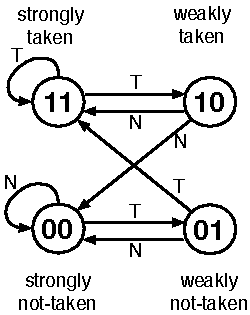
\includegraphics[scale =1] {figures/2bc-fsm}}
	\caption{ \small Two-bit counter state machine.}
	\label{fig:2bc-fsm}
\end{figure}

Although it's no longer strictly a ``counter", this change allows us to separate out the read and write requirements on the {\em prediction} and {\em hystersis} bits and place them in separate sequential memory tables. In hardware, the 2bc table can be implemented as follows:

\begin{quote}
The P-bit:
\begin{itemize}
\item {\bf read} - every cycle to make a prediction
\item {\bf write} - only when a misprediction occurred (the value of the h-bit).
\end{itemize}

The H-bit:

\begin{itemize}
\item {\bf read} - only when a misprediction occurred.
\item {\bf write} - when a branch is resolved (write the direction the branch took).
\end{itemize}
\end{quote}

By breaking the high-order p-bit and the low-order h-bit apart, we can place each in 1 read/1write SRAM. A few more assumptions can help us do even better. Mispredictions are rare and branch resolutions are not necessarily occurring on every cycle. Also, writes can be delayed or even dropped altogether. Therefore, the {\em h-table} can be implemented using a single 1rw ported SRAM by queueing writes up and draining them when a read is not being performed. Likewise, the {\em p-table} can be implemented in 1rw ported SRAM by banking it -- buffer writes and drain when there is not a read conflict.


A final note: SRAMs are not happy with a ``tall and skinny'' aspect ratio that the 2bc tables require. However, the solution is simple -- tall and skinny can be trivially transformed into a rectangular memory structure.  The high-order bits of the index can correspond to the SRAM row and the low-order bits can be used to mux out the specific bits from within the row. 

\subsection{The GShare Predictor}

GShare is a simple but very effective branch predictor. Predictions are made by hashing the instruction address and the global history (typically a simple XOR) and then indexing into a table of two-bit counters. 

\subsection{The TAGE Predictor}\label{sec:tage}

\TODO{...}

\subsection{Other Predictors}

BOOM provides a number of other predictors that may provide useful.

\subsubsection{The Null Predictor}

The Null Predictor is used when no BPD predictor is desired. It will always predict ``not taken".

\subsubsection{The Random Predictor}

The Random Predictor uses an LFSR to randomize both ``was a prediction made?" and ``which direction each branch in the {\em fetch packet} should take?".  This is very useful for both torturing-testing BOOM and for providing a worse-case performance baseline for comparing branch predictors.

\section{Branch Prediction Configurations}

There are a number of parameters provided to govern the branch prediction in BOOM.

\TODO{...}
 

\include{sections/decode}
\include{sections/rename}
\include{sections/rob}
\include{sections/issue}
\include{sections/registerread}
\include{sections/execute}

\chapter{The Load/Store Unit (LSU)}\label{sec:lsu}

The Load/Store Unit is responsible for deciding when to fire memory operations to the memory system.  There are three queues: the Load Address Queue (LAQ), the Store Address Queue (SAQ), and the Store Data Queue (SDQ).  Load instructions generate a ``uopLD" micro-op.  When issued, ``uopLD" calculates the load address and places its result in the LAQ.  Store instructions (may) generate {\em two} micro-ops,  ``uopSTA" (Store Address Generation) and ``uopSTD" (Store Data Generation).  The STA micro-op calculates the store address and places its result in the SAQ queue.  The STD micro-op moves the store data from the register file to the SDQ.  Each of these micro-ops will issue out of the {\em Issue Window} as soon their operands are ready.  See Section \ref{sec:storeuops} for more details on the store micro-op specifics. 



\section{Store Instructions}

Entries in the Store Queue\footnote{When I refer to the {\em Store Queue}, I really mean both the SAQ and SDQ.} are allocated in the {\em Decode} stage (the appropriate bit in the {\tt stq\_entry\_val} vector is set).  A ``valid" bit denotes when an entry in the SAQ or SDQ holds a valid address or data ({\tt saq\_val} and {\tt sdq\_val} respectively).  Once a store instruction is committed, the corresponding entry in the Store Queue is marked as committed.  The store is then free to be fired to the memory system at its convenience.  Stores are fired to the memory in program order.


\subsection{Store Micro-ops}\label{sec:storeuops}

Stores are inserted into the issue window as a single instruction (as opposed to being broken up into separate {\tt addr-gen} and {\tt data-gen} micro-ops). This prevents wasteful usage of the expensive issue window entries and extra contention on the issue port to the LSU.  A store in which both operands are ready can be issued to the LSU as a single micro-op which provides both the address and the data to the LSU.  While this requires store instructions to have access to two register file read ports, this is motivated by a desire to not cut performance in half on store-heavy code.  Sequences involving stores to the stack should operate at IPC=1!

However, it is common for store addresses to be known well in advance of the store data.  Store addresses should be moved to the SAQ as soon as possible to allow later loads to avoid any memory ordering failures. Thus, the issue window will emit uopSTA or uopSTD micro-ops as required, but retain the remaining half of the store until the second operand is ready.

\section{Load Instructions}

Entries in the Load Queue (LAQ) are allocated in the {\em Decode} stage ({\tt laq\_entry\_val}).  In {\em Decode}, each load entry is also given a {\em store mask} ({\tt laq\_st\_mask}), which marks which stores in the Store Queue the given load depends on.  When a store is fired to memory and leaves the Store Queue, the appropriate bit in the {\em store mask} is cleared.

Once a load address has been computed and placed in the LAQ, the corresponding {\em valid} bit is set ({\tt laq\_val}). 

Loads are optimistically fired to memory on arrival to the LSU (getting loads fired early is a huge benefit of out--of--order pipelines).  Simultaneously, the load instruction compares its address with all of the store addresses that it depends on.  If there is a match, the memory request is killed.  If the corresponding store data is present, then the store data is {\em forwarded} to the load and the load marks itself as having {\em succeeded}.  If the store data is not present, then the load goes to {\em sleep}.  Loads that have been put to sleep are retried at a later time.\footnote{Higher-performance processors will track {\em why} a load was put to sleep and wake it up once the blocking cause has been alleviated.}



\section{The BOOM Memory Model}

Currently, as of October 2016, the RISC-V memory model is underspecified and will take some time to settle on an exact specification. However, the current RISC-V specification describes as {\em relaxed consistency} model~\cite{Gharachorloo:1990:MCE:325096.325102} in which stores and loads may be freely re-ordered. 

BOOM currently exhibits the following behavior:

\begin{enumerate}
\item Write->Read constraint is relaxed (newer loads may execute before older stores).
\item Read->Read constraint is currently relaxed (loads to the same address may be reordered). 
\item A thread can read its own writes early. 
\end{enumerate}


\subsection{Ordering Loads to the Same Address}

The RISC-V memory model is expected to strengthen the requirement that loads to the same address be ordered.\footnote{Technically, a {\em fence.r.r} could be used to provide the correct execution of software on machines that reorder dependent loads. However, there are two reasons for an ISA to disallow re-ordering of dependent loads: 1) no other popular ISA allows this relaxation, and thus porting software to RISC-V could face extra challenges, and 2) cautious software may be too liberal with the appropriate {\em fence} instructions causing a slow-down in software. Thankfully, enforcing ordered dependent loads may not actually be very expensive. For one, load addresses are likely to be known early - and are probably likely to execute in-order anyways. Second, misordered loads are only a problem in the cache of a cache coherence probe, so performance penalty is likely to be negligible. The hardware cost is also negligible - loads can use the same CAM search port on the LAQ that stores must already use.  While this may become an issue when supporting one load and one store address calculation per cycle, the extra CAM search port can either be mitigated via banking or will be small compared to the other hardware costs required to support more cache bandwidth.} This requires loads to search against other loads for potential address conflicts. If a younger load executes before an older load with a matching address, the younger load must be replayed and the instructions after it in the pipeline flushed. However, this scenario is only required if a cache coherence probe event snooped the core's memory, exposing the reordering to the other threads.  If no probe events occurred, the load re-ordering may safely occur. 


\section{Memory Ordering Failures}

The Load/Store Unit has to be careful regarding {\tt store$\rightarrow$load} dependences.  For the best performance, loads need to be fired to memory as soon as possible. 

\begin{quote}

{\texttt
sw x1 $\rightarrow$ 0(x2)

ld x3 $\leftarrow$ 0(x4)
}

\end{quote}


However, if {\tt x2} and {\tt x4} reference the same memory address, then the load in our example {\em depends} on the earlier store.  If the load issues to memory before the store has been issued, the load will read the wrong value from memory, and a {\em memory ordering failure} has occurred.  On an ordering failure, the pipeline must be flushed and the rename map tables reset.  This is an incredibly expensive operation.

To discover ordering failures, when a store commits, it checks the entire LAQ for any address matches.  If there is a match, the store checks to see if the load has {\em executed}, and if it got its data from memory or if the data was forwarded from an older store.  In either case, a memory ordering failure has occurred.  

See Figure \ref{fig:lsu} for more information about the Load/Store Unit.

\


\begin{figure}[ht]
	\centering
	\centerline{\includegraphics[scale =.9] {figures/lsu}}
	\caption{ \small The Load/Store Unit.}
	\label{fig:lsu}
\end{figure}


\include{sections/memory}
\chapter{Micro-architectural Event Tracking}

Version 1.9.1 of the RISC-V Privileged Architecture adds support for Hardware Performance Monitor (HPM) counters.\footnote{Future efforts may add some counters into a memory-mapped access region. This will open up the ability to track events that, for example, may not be tied to any particular core (like last-level cache misses).}  The HPM support allows a nearly infinite number of micro-architectural events to be multiplexed onto up to 29 physical counters.  The privilege access levels can also be set on a per-counter basis.

\begin{table}[htp]
\caption{Uarch Events}
\begin{center}
\begin{tabular}{|c|c|}
\hline
Number & Event \\
\hline
\hline
1 & Committed Branches  \\
\hline
2 & Committed Branch Mispredictions\\
\hline
... & and many more (see core.scala) \\
\hline
\end{tabular}
\end{center}
\label{table:uarchcounters}
\end{table}%

The available events can be modified in {\tt core.scala} as desired.\footnote{Note: {\tt io.events(0)} will get mapped to being {\tt Event \#1} (etc.) from the point of view of the RISC-V software.}  It is then up to machine-level software to set the privilege access level and the {\em event selectors} for each counter as desired.

\begin{center}
\begin{minipage}{0.66\textwidth}
\begin{lstlisting}[caption=Setting the privilege level and event selectors for the HPM counters.]
static void mstatus_init()
{
   // Enable user/supervisor use of perf counters
   write_csr(mucounteren, -1);
   write_csr(mscounteren, -1);

   // set events 1 and 2 to counters 3 and 4.
   write_csr(mhpmevent3, 1);
   write_csr(mhpmevent4, 2);
\end{lstlisting}\label{ref:code_hpm_init}
\end{minipage}
\end{center}


\section{Reading HPM Counters in Software}

The Code Example \ref{ref:code_uarch} demonstrates how to read the value of any CSR register from software.
  
  
\begin{center}
\begin{minipage}{0.66\textwidth}
\begin{lstlisting}[caption=Reading a CSR register.]
#define read_csr_safe(reg) ({ register long __tmp asm("a0"); \   
  asm volatile ("csrr %0, " #reg : "=r"(__tmp)); \               
  __tmp; })             
  
  long csr_cycle  = read_csr_safe(cycle);
  long csr_instr  = read_csr_safe(instret);
  long csr_hpmc3  = read_csr_safe(hpmcounter3);
  ...
  long csr_hpmc31 = read_csr_safe(hpmcounter31);
  
\end{lstlisting}\label{ref:code_uarch}
\end{minipage}
\end{center}



\include{sections/verification}
\chapter{Debugging}
\include{sections/visualization}
\chapter{Physical Realization}\label{chapter:physical}

This chapter provides information useful for physically realizing the BOOM processor.  Although BOOM VLSI work is very preliminary, it has been synthesized at 1~GHz on a high-end mobile 28~nm process. Unfortunately, while VLSI flows are difficult to share or make portable (and encumbered with proprietary libraries and tools), an enterprising individual may want to visit the \url{https://github.com/ucb-bar/plsi} portable ``Palmer's VLSI Scripts'' repository which describes one way to push BOOM through a VLSI flow.

\section{Register Retiming}
 
Many VLSI tools require the designer to manually specify which modules need to
be analyzed for retiming. 
                 
In BOOM, the floating point units and the pipelined integer multiply unit are
described combinationally and then padded to the requested latency with
registers.
In order to meet the desired clock frequency,  {\bf the floating point units and the
pipelined integer multiply unit must be register-retimed}.
 
\begin{center}
\begin{minipage}{0.90\textwidth}
\begin{lstlisting}[caption=Pipelined integer multiply unit requires register retiming to be realized properly.]
val mul_result = lhs.toSInt * rhs.toSInt
                                                                               
val mul_output_mux = MuxCase(                                                  
   UInt(0, 64), Array(                                                         
      FN(DW_64, FN_MUL)    -> mul_result(63,0),                                
      FN(DW_64, FN_MULH)   -> mul_result(127,64),                              
      FN(DW_64, FN_MULHU)  -> mul_result(127,64),                              
      FN(DW_64, FN_MULHSU) -> mul_result(127,64),                              
      FN(DW_32, FN_MUL)    -> Cat(Fill(32, mul_result(31)), mul_result(31,0)), 
      FN(DW_32, FN_MULH)   -> Cat(Fill(32, mul_result(63)), mul_result(63,32)),
      FN(DW_32, FN_MULHU)  -> Cat(Fill(32, mul_result(63)), mul_result(63,32)),
      FN(DW_32, FN_MULHSU) -> Cat(Fill(32, mul_result(63)), mul_result(63,32)) 
))                                                                             
                                                                               
io.out := ShiftRegister(mul_output_mux, imul_stages, io.valid)
\end{lstlisting}\label{code:imul}
\end{minipage}
\end{center}

\section{Pipelining Configuration Options}

Although BOOM does not provide high-level configurable-latency pipeline stages, BOOM does provide a few configuration options to help the implementor trade off CPI performance for cycle-time. 

\subsubsection{EnableFetchBufferFlowThrough}

The front-end fetches instructions and places them into a {\em fetch buffer}.  The back-end pulls instructions out of the fetch buffer and then decodes, renames, and dispatches the instructions into the {\em issue window}. This fetch buffer can be optionally set to be a {\em flow-through} queue -- instructions enqueued into the buffer can be immediately dequeued on the other side on the same clock cycle.  Turning this option {\bf off} forces all instructions to spend at least one cycle in the queue but decreases the critical path between instruction fetch and dispatch.

\subsubsection{EnableBrResolutionRegister}

The branch unit resolves branches, detects mispredictions, fans out the branch kill signal to {\em all} inflight micro-ops, redirects the PC select stage to begin fetching down the correct path, and sends snapshot information to the branch predictor to reset its state properly so it can begin predicting down the correct path.  Turning this option {\bf on} delays the branch resolution by a cycle.  In particular, this adds a cycle to the branch misprediction penalty (which is hopefully a rare event).

\subsubsection{Functional Unit Latencies}

The latencies of the pipelined floating point units and the pipelined integer multiplier unit can be modified.  Currently, all floating point unit latencies are set to the latency of the longest floating point unit (i.e., the DFMA unit).  This can be changed by setting the {\em dfmaLatency} in the {\em FPUConfig} class. Likewise, the integer multiplier is also set to the {\em dfmaLatency}.\footnote{The reason for this is that the imul unit is most likely sharing a write port with the DFMA unit and so must be padded out to the same length. However, this isn't fundamental and there's no reason an imul unit not sharing a write port with the FPUs should be constrained to their latencies.}


\appendix
\chapter{Future Work}

This chapter lays out some of the potential future directions that BOOM can be taken.  To help facilitate such work, the preliminary design sketches are described below. 

\section{The Rocket Custom Co-processor Interface (ROCC)}

The Rocket in-order processor comes with a ROCC interface that facilitates communication with co-processor/accelerators.  Such accelerators include crypto units (e.g., SHA3) and vector processing units (e.g., the open-source Hwacha vector-thread unit\cite{hwacha}). 

The ROCC interface accepts co-processor commands emitted by {\em committed} instructions run on the ``Control Processor" (e.g., a scalar Rocket core).  Any ROCC commands {\em will} be executed by the co-processor (barring exceptions thrown by the co-processor); nothing speculative can be issued over ROCC. 

Some ROCC instructions will write back data to the Control Processor's scalar register file. 

\subsection{The Demands of the ROCC Interface}


The ROCC interface accepts a ROCC command and up to two register inputs from the Control Processor's scalar register file. 
The ROCC command is actually the entire RISC-V instruction fetched by the Control Processor (a ``ROCC instruction"). Thus, each ROCC queue entry is at least 2*XPRLEN + 32 bits in size (additional ROCC instructions may use the longer instruction formats to encode additional behaviors). \TODO{draw a diagram showing this}

As BOOM does not store the instruction bits in the ROB, a separate data structure (A ``ROCC Reservation Station") will have to hold the instructions until the ROCC instruction can be committed and the ROCC command sent to the co-processor. 

The source operands will also require access to BOOM's register file.  Two possibilities are proposed:

\begin{itemize}
\item ROCC instructions are dispatched to the Issue Window, and scheduled so that they may access the read ports of the register file once the operands are available. The operands are then written into the ROCC Reservation Station, which stores the operands and the instruction bits until they can be sent to the co-processor.  This may require significant state. 
\item ROCC instructions, when they are committed and sent to the ROCC command queue, must somehow access the register file to read out its operands.  If the register file has dynamically scheduled read ports, this may be trivial. Otherwise, some technique to either inject a ROCC micro-op into the issue window or a way to stall the issue window while ROCC accesses the register file will be needed. 
\end{itemize}


\subsection{A Simple One-at-a-Time ROCC Implementation}

The simplest way to add ROCC support to BOOM would be to stall {\em Decode} on every ROCC instruction and wait for the ROB to empty.  Once the ROB is empty, the ROCC instruction can proceed down the BOOM pipeline non-speculatively, and get sent to the ROCC command queue.  BOOM remains stalled until the ROCC accelerator acknowledges the completion of the ROCC instruction and sends back any data to BOOM's register file. Only then can BOOM proceed with its own instructions. 


\subsection{A High-performance ROCC Implementation Using Two-Phase Commit}

While some of the above constraints can be relaxed, the performance of a decoupled co-processor depends on being able to queue up multiple commands while the Control Processor runs ahead (prefetching data and queueing up as many commands as possible).  However, this requirement runs counter to the idea of only sending committed ROCC instructions to the co-processor. 

BOOM's ROB can be augmented to track {\em commit} and {\em non-speculative} pointers. The {\em commit} head pointer tracks the next instruction that BOOM will {\em commit}, i.e., the instruction that will be removed from the ROB and the resources allocated for that instruction will be de-allocated for use by incoming instructions. The {\em non-speculative} head will track which instructions can no longer throw an exception and are no longer speculated under a branch (or other speculative event), i.e., which instructions absolutely will execute and will not throw a pipeline-retry exception. 

This augmentation will allow ROCC instructions to be sent to the ROCC command queue once they are deemed ``non-speculative", but the resources they allocate will not be freed until the ROCC instruction returns an acknowledgement.  This prevents a ROCC instruction that writes a scalar register in BOOM's register file from overwriting a newer instruction's writeback value, a scenario that can occur if the ROCC instruction commits too early, followed by another instruction committing that uses the same ISA register as its writeback destination. 


\subsection{The BOOM Custom Co-processor Interface (BOCC)}

Some accelerators may wish to take advantage of speculative instructions (or even out-of-order issue) to begin executing instructions earlier to maximize de-coupling.  Speculation can be handled by either by epoch tags (if in-order issue is maintained to the co-processor) or by allocating mask bits (to allow for fine-grain killing of instructions). 

\section{The Vector (``V") ISA Extension}

Implementing the Vector Extension in BOOM would open up the ability to leverage performance (or energy-efficiency) improvements in running data-level parallel codes (DLP).  While it would be relatively easy to add vector arithmetic operations to BOOM, the significant challenges lie in the vector load/store unit. 

Perhaps unexpectedly, a simple but very efficient implementation could be very small.  The smallest possible vector register file (four 64-bit elements per vector) weighs in at 1024 bytes.  A reasonable out-of-order implementation could support 8 elements per vector and 16 inflight vector registers (for a total of 48 physical vector registers) which would only be 3 kilobytes.  Following the temporal vector design of the Cray I, the vector unit can re-use the expensive scalar functional units by trading off space for time.  This also opens up the vector register file to being implemented using 1 read/1 write ports, fitting it in very area-efficient SRAMs.  As a point of comparison, the one of the most expensive parts of a synthesizable BOOM is its flip-flop based scalar register file.  While a 128-register scalar register file comes in at 1024 bytes, it must be highly ported to fully exploit scalar instruction-level parallelism (a three-issue BOOM with one FMA unit is 7 read ports and 3 write ports).


\section{The Compressed (``C") ISA Extension}

This section describes how to approach adding the Compressed ISA Extension to BOOM.  The Compressed ISA Extension, or RVC  (\url{http://riscv.org/download.html#spec_compressed_isa}) enables smaller, 16 bit encodings of common instructions to decrease the static and dynamic code size.  ``RVC" comes with a number of features that are of particular interest to micro-architects:

\begin{itemize}
\item All 16b instructions map directly into a longer 32b instruction. 
\item 32b instructions have no alignment requirement, and may start on a half-word boundary.
\end{itemize}

\begin{figure}[ht]
	\centering
	\centerline{\includegraphics[scale =1] {figures/frontend}}
	\caption{ \small The Fetch Unit. The grey box encompasses the Rocket front-end, which is re-used by BOOM.}
	\label{fig:futurework-frontend}
\end{figure}

BOOM re-uses the front-end design from Rocket, a 5-stage in-order core.  BOOM then takes instructions returning (the {\em fetch packet}) from the Rocket front-end, quickly decodes the instructions for branch prediction, and pushes the {\em fetch packet} into the {\em Fetch Buffer}. 


The C Extension provides the following challenges to micro-architects, a few include:

\begin{itemize}
\item Increased decoding complexity (e.g., operands can now move around). 
\item Finding {\em where} the instruction begins. 
\item Tracking down $+4$ assumptions throughout the code base, particularly with branch handling.
\item Unaligned instructions, in particular, running off cache lines and virtual pages. 
\end{itemize}

The last point requires some additional ``statefulness" in the Fetch Unit, as fetching all of the pieces of an instruction may take multiple cycles. 

The following describes the proposed implementation strategy of RVC in BOOM:

\begin{itemize}
\item Implement RVC in the Rocket in-order core.  Done properly, BOOM may then gain RVC support almost entirely for free (modulo any $+4$ assumptions in the code base).
\item Move BOOM's {\em Fetch Buffer} into Rocket's front-end. Rocket will need the statefulness to handle wrap-around issues with fetching unaligned 32 bit instructions.  A non-RVC Rocket core can optionally remove this buffer. 
\item Expand 16-bit instructions as they enter (or possibly exit) the {\em Fetch Buffer}. 
\item Minimize latency by placing 16b$\rightarrow$32b expanders at every half-word start. 
\end{itemize}

\subsection{Challenging Implementation Details}

There are many challenging corner cases to consider with adding RVC support to BOOM. First, although all 16 bit encodings map to a 32b version, {\bf the behavior of some 16b instructions are different from their 32b counterparts}!  A JAL instruction writes the address of the following instruction to {\tt rd} - but whether that is $PC+2$ or $PC+4$ depends on whether it's the 16b JAL or a 32b JAL!  Likewise, a mispredicted not-taken branch redirects the fetch unit to $PC+2$ or $PC+4$ depending on whether the branch was the compressed version or not. {\bf Thus, the pipeline must track whether any given instruction was originally a compressed 16b instruction or not.}

The branch prediction units will also require a careful rethink. The BTB tracks which instructions are {\em predicted-taken} branches and redirects the PC as desired. For a superscalar {\em fetch packet}, the BTB must help denote which instruction is to be blamed for the taken prediction to help mask off any invalid instructions that come afterward within the {\em fetch packet}. RVC makes this much more difficult, as some {\em predicted-taken} branches can wrap around fetch groupings/cache lines/virtual page boundaries. Thus, the ``taken" prediction must be attached to a tag-hit on the {\em end} of the branch instruction.  This handles fetching the first part of the branch (and predicting ``not-taken"), then fetching the second part (which hits in the BTB and predicts ``taken"), and only then redirecting the front-end to the predicted-taken PC target. 

%TODO is this a problem?
%One final detail to keep in mind is the potential interactions of the i-cache and the instruction translation look-aside buffer (i-TLB) with regards to self-modifying RVC code.  A RISC-V instruction can legally straddle a virtual page boundary such that the second half is neither in the i-cache nor in the i-TLB. A self-modifying program could store out new instructions that are not resident in the i-cache (or i-TLB).  However, such a store could override the last half 

\include{sections/parameterization}

\chapter{Frequently Asked Questions}

To be filled in as questions are asked!

\include{sections/terminology}


\begin{figure}[ht]
	\centering
	\centerline{\includegraphics[scale =.9, angle=90] {figures/simple_boom_pipeline}}
	\caption{ \small A more detailed diagram of BOOM, for a single-issue RV32IM design.}
	\label{fig:boom-detailed}
\end{figure}






%\begin{scriptsize}
\bibliographystyle{abbrv}
\bibliography{bibliography}
%\end{scriptsize}


\end{document}
